\documentclass{sigchi}

% Use this command to override the default ACM copyright statement (e.g. for preprints). 
% Consult the conference website for the camera-ready copyright statement.
\toappear{
	Submitted for review.
}

% Arabic page numbers for submission. 
% Remove this line to eliminate page numbers for the camera ready copy
\pagenumbering{arabic}


% Load basic packages
\usepackage{balance}  % to better equalize the last page
\usepackage{graphics} % for EPS, load graphicx instead
\usepackage{times}    % comment if you want LaTeX's default font
\usepackage{url}      % llt: nicely formatted URLs

\usepackage{textcomp}


% llt: Define a global style for URLs, rather that the default one
\makeatletter
\def\url@leostyle{%
  \@ifundefined{selectfont}{\def\UrlFont{\sf}}{\def\UrlFont{\small\bf\ttfamily}}}
\makeatother
\urlstyle{leo}


% To make various LaTeX processors do the right thing with page size.
\def\pprw{8.5in}
\def\pprh{11in}
\special{papersize=\pprw,\pprh}
\setlength{\paperwidth}{\pprw}
\setlength{\paperheight}{\pprh}
\setlength{\pdfpagewidth}{\pprw}
\setlength{\pdfpageheight}{\pprh}

% Make sure hyperref comes last of your loaded packages, 
% to give it a fighting chance of not being over-written, 
% since its job is to redefine many LaTeX commands.
\usepackage[pdftex]{hyperref}
\hypersetup{
pdftitle={Augmented Reality Tools for 
  the Creation of Physical Visual Arts},
pdfauthor={LaTeX},
pdfkeywords={mixed reality, projection mapping, drawing, touch input},
bookmarksnumbered,
pdfstartview={FitH},
colorlinks,
citecolor=black,
filecolor=black,
linkcolor=black,
urlcolor=black,
breaklinks=true,
}

% create a shortcut to typeset table headings
\newcommand\tabhead[1]{\small\textbf{#1}}

% End of preamble. Here it comes the document.
\begin{document}

\title{Mixed drawing - merging physical drawing with creative coding}

%\numberofauthors{1}
%\author{
%  \alignauthor 1st Author Name\\
%    \affaddr{Affiliation}\\
%    \affaddr{Address}\\
%    \email{e-mail address}\\
%}

 \numberofauthors{2}
 \author{
   \alignauthor 1st Author Name\\
     \affaddr{Affiliation}\\
     \affaddr{Address}\\
     \email{e-mail address}\\
   \alignauthor 2nd Author Name\\
     \affaddr{Affiliation}\\
     \affaddr{Address}\\
     \email{e-mail address}\\
 }



%% \begin{figure*}[th]
%% \centering
%% 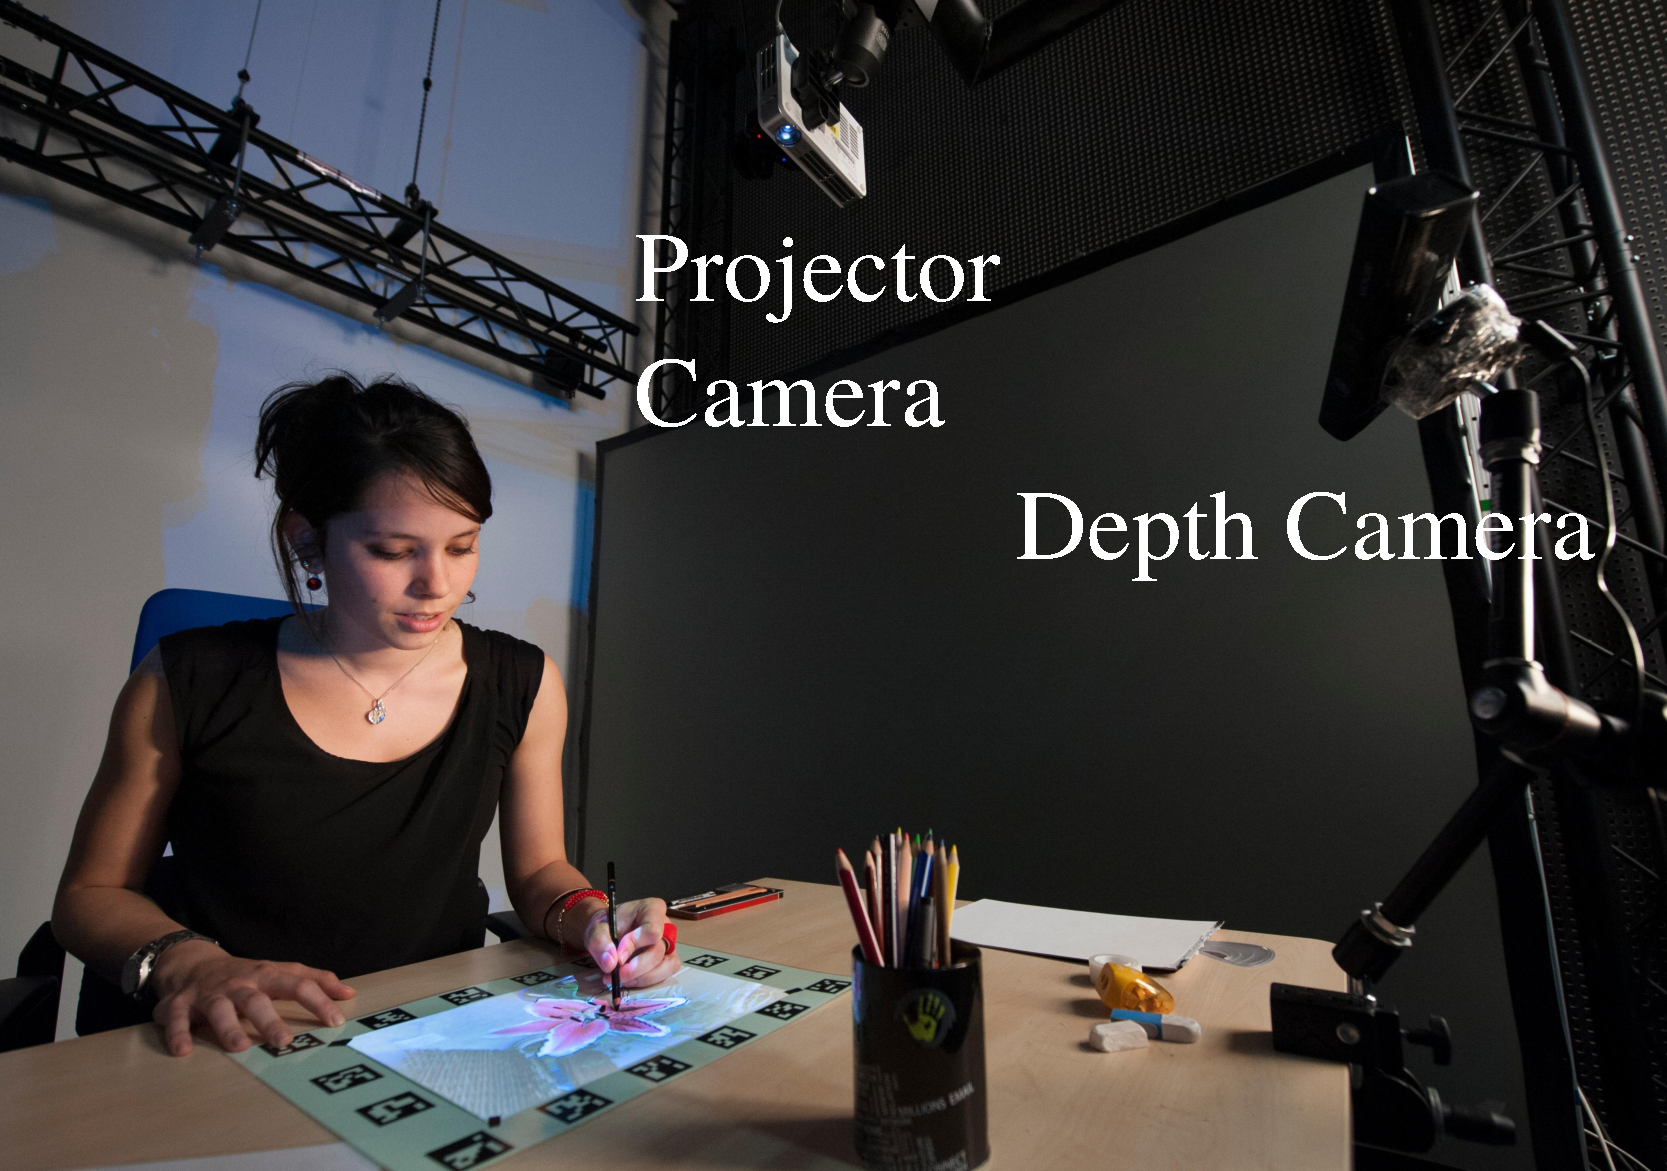
\includegraphics[width=85mm]{systempro.pdf}
%% \caption{Projection mapping resulting system.}
%% \label{fig:teaser}
%% \end{figure*}





\maketitle
 

%\vspace{55mm}
%
\includegraphics[height=55mm]{teaser.pdf}

\begin{abstract}

\end{abstract}


\keywords{mixed reality, projection mapping, creative coding, drawing, touch input}
% \vspace{-0.15cm}


\category{H.5.1}{Information interfaces and presentation}{Information interfaces and presentation}
% \vspace{-0.15cm}

\terms{Design, Human Factors}
% \vspace{-0.15cm}

%% \keywords{
%% 	augmented reality; projection mapping; drawing; painting; non
%%         photorealistic rendering
%% }

\section{Introduction}

Creative coding the
action of writing code not only for pleasure but also without any
purposes except aestetics of entertainment.  It emerged with the first
computers programs. The results of the programs were at first purely
digital; nowadays it is possible to print them as images, 3D objects
or apparel (cite...).

However, it is intersting to keep the programs running in order to obtain an
interactive experience. The creation of mixed mediums, using drawings
and sculpture with projection has been explored by artists in the past
few years. The creation of such pieces of art requires time and
dedication, consequently the results are usually animations and rarely
interactive. In this paper we focus on the easy creation of planar
(2D) interactive mixed drawings. 

We enable the users to manipulate 
directly images, videos and programs using a touch and tangible
interface in a spatial augmented reality setup. 

\section{Related works}

We built our tool over the popular creative coding solution
Processing (cite). Processing is a language and IDE based on Java, it
was created for creative coding by Casea Reas and Ben Fry (cite). 

The emergence of this kind of simple programming languages enables
programming to anyone without a computer science background. 
In this paper it is out target audience, we enable them to ``compose'' 
programs made of multiple processing sketches, images and videos. 

-- Related works dans la composition 

-- Revoir Touch \& Tangible biblio dans le papier precedent... 


\section{Technical setup}



\begin{itemize}
\item SAR - markers, projection  (main paper + additional cardboards)
\item Touch - Kinect
\item Capture - additional Camera	 
\item Processing
\end{itemize}

\section{Mixing physical and digital drawing}

\subsection{Layer representation} 

The first basic tools we propose is to compose the drawing with images
and videos. The user can choose which one to integrate and then place
them using the touch interface. 
We use the same interface to add programs (``Processing sketches''). 
Videos, Programs or Images will be referred as Layers. 

We propose to use a hierarchical ordering of the layers as a tree: 
there is a root layer, containing sub-layers, and each sub-layer could
also have sub-layers. The tree representation is fundamental in
computer science: the position in the structure of will influence the
layer's position and rendering. 

\subsection{Writing a program for the physical world}

In computer graphics, everything is pixel or algorithms. However, in
the real world pixels can be more or less dense and algorithms need a
scale to be rendered. Consequently, the programmer must specify not
only the size in pixels of the sketch, but also the size in
millimeters. This size is not definitive, a program is a common layer:
it can be moved and resized at will. 

We tried to maintain the writing of programs as close as possible to
usual Processing sketches. The first change was the addition of a
physical size, the second change is the choice in the input method. 
We propose two input methods, either the touch or the 3d input, the
user can switch between the two. The program will receive in priority
the events in its drawing area, then the events outside it (like
events outside a window in any operating system). 
The events are mapped to the values \texttt{mouseX}, \texttt{mouseY},
\texttt{pmouseX} and \texttt{pmouseY} (mouse current and previous
position) so that any sketch using the mouse will
easily work in the projected environment. 

Figure ... shows the difference between a Processing sketch and a
sketch with our solution. 

-- Figure ... 


The composition of programs as layers enables an easy manipulation
that could stimulate the creative process. Here is an example: we want
to create mixed scene with a car, the car is drawn and the wheels and
background are programs and create the illusion of movement. 
The user have to create one program for the wheels, invoke it two
times, and then place each wheels in a ``What You See Is What You
Get'' (WYSIWYG) way. He or she creates also a scrolling background
program, and also invoke it multiple times. Once everything is in
place, at the right scale and positions, it is possible to measure the
result to adujst the programs or just keep them running. 

--- Figure : rolling car... 

\subsection{Interaction between programs}

We mentionned earlier that the programs are running as layers, they
cannot interfere with each other's positions or access the underlying
layer structure. The communication can be achived using variables
outside the SubSketch class (Figure ...). Like in any Processing
sketch the variables are accessible to all files, here they are
accessible to every SubSketch. 

We propose an example use of this to control the wheather in a mixed
drawing. We took a few sketches from OpenProcessing.org, one for
snow (cite...) and one for fire. We wrote a third program to control
the two former. The third program has three switches depending on
where the user moves the ``mouse'', which is replaced by the touch
interface. We propose to replace the finger interaction by a small
paper cube to control the wheather. As we mentionned before, each
program takes in priority the touch inside it. Consequently, 
the small programs controlled by tangible objects will generally not
influence tactile-sensitive programs. 

--- Figure : cube feu - neige.

\section{Interactive edition of the rendering}

The rendering of a layer can be interactively changed by applying
filters. Each filter can be applied to the whole layer or part of
it. Which part to filter is edited by touching the zone to
filter. However, our implementation is a ``proof of concept'' and does
not provide a set of brushes like most of the painting tools.

The creation of these filters is for advanced programmers (GLSL
shaders), but their use is very simple. Every filter can be added any
number of time to a layer and its sublayers. Consequently, its effects
can be increased (for a blur filter), or it can be used to push the
limits of the filters and create new uses out of it. 

We demonstrate the use of filters with a scene inspired ...




\subsection{Creating animated drawings}
\begin{itemize}
  \item animated sequences 
\end{itemize}

\section{User feedback and discussion}

on demande de faire un dessin qui necessite l'utilisation de ''Digital tools for traditional drawing''
on voit ce qu'ils en disent. On discute.


\section{Conclusion}

 
\balance

% If you want to use smaller typesetting for the reference list,
% uncomment the following line:
%\small
\bibliographystyle{acm-sigchi}
\bibliography{biblio}


\end{document}
